%% Standard-Vorspann
\documentclass[a4paper,11pt,twoside]{report}
\usepackage{ngerman}  
\usepackage[utf8]{inputenc}                
%\usepackage[latin1]{inputenc}
\usepackage[T1]{fontenc}
\usepackage[fleqn]{amsmath}
\usepackage{mathtools}
\usepackage{bm}
\DeclarePairedDelimiter\ceil{\lceil}{\rceil}
\DeclarePairedDelimiter\floor{\lfloor}{\rfloor}

%% Auf Schriftart Palatino umschalten
\usepackage{mathpazo}
\usepackage[scaled=.95]{helvet}
\usepackage{courier}
\usepackage[figuresright]{rotating}
%% fast immer benoetigte Pakete
\usepackage{acronym}
\usepackage{amssymb, amsthm}
\usepackage{alltt}
\usepackage{latexsym}
\usepackage{makeidx}
\usepackage{textcomp}
\usepackage{rotating}
\usepackage{color}
\usepackage[table]{xcolor}
\usepackage{caption}
\usepackage{listings}
\usepackage{verbatim}
\usepackage{fancyhdr}
\usepackage{graphicx}
\usepackage{subcaption}
\usepackage{thmtools}
\declaretheorem[style=Definition, title=Definition, numberwithin=chapter]{dfn}
\newtheorem{axiom}{Axiom}
\usepackage{tikz}
\usepackage{multirow}
\usepackage[natbib,maxnames=3,style=numeric,backend=bibtex,sortlocale=de]{biblatex}
\addbibresource{bibtex/literature.bib}
\DeclareBibliographyCategory{fullcited}
\usepackage{listings}
\usepackage[hang]{footmisc}
\usepackage{chngcntr}
\counterwithout{footnote}{chapter}
\setlength{\footnotemargin}{0pt}
\usepackage{url}
\renewcommand\UrlFont{\sffamily\slshape}
\usepackage{nicefrac}
\usepackage{units}
\usepackage{minibox}
\pdfminorversion=7
\usepackage{emptypage}
\usepackage{hyperref}

%% spezielles Zeug
\usepackage{Abschlussarbeit}


%
\chapter{Abk\"urzungsverzeichnis}

% ======================================================================
% Declare acronyms
% ======================================================================

\begin{acronym}
	\acro{ARRI}[ARRI]{Arnold \& Richter Cine Technik GmbH \& Co. Betriebs KG}
	\acro{fpga}[FPGA]{Field Programmable Gate Array}
	\acro{fra}[FRA]{FPGA Resource Abstraction}
	\acro{geo}[Geo Framework]{Geometrie Framework}
	\acro{gui}[GUI]{grafische Benutzeroberfläche}
	\acro{ioctl}[IOCTL]{IO Control}
	\acro{mfd}[MFD]{Multifunction Device}
	\acro{rec}[REC]{Aufnahme}
	\acro{pid}[PID]{Prozesskennung}
	\acro{smpte}[SMPTE]{Society of Motion Picture and Television Engineers}
	\acro{sdi}[SDI]{Serial Digital Interface} gemäß \ac{smpte} 292M \footnote{\url{https://ieeexplore.ieee.org/document/7291770}}
	\acro{xbar}[Xbar]{Crossbar}
\end{acronym}



%% Index erzeugen
\makeindex

%% jetzt geht's los
\begin{document}
\raggedbottom
\hypersetup{
	colorlinks,
	citecolor=black,
	filecolor=black,
	linkcolor=black,
	urlcolor=black
}

\definecolor{mygreen}{rgb}{0,0.6,0}
\definecolor{mygray}{rgb}{0.5,0.5,0.5}
\definecolor{mymauve}{rgb}{0.58,0,0.82}

\lstset{language=C,
		basicstyle=\footnotesize,
		commentstyle=\color{mygreen},
		keywordstyle=\color{blue},
		numbers=left,
		numbersep=5pt,
		numberstyle=\tiny\color{mygray},
		breakatwhitespace=false,
		tabsize=2,	
		frame=single, %todo ja oder nein??
		breaklines=true}
\captionsetup[lstlisting]{font=it,
						  position=below,
					  	  belowskip=0.5cm}

%% Die Datei "Vorspann.tex"  bitte ausf�llen!
% Vorspann der Arbeit
%

\includegraphics[width=45mm]{pictures/Hochschule_Muenchen_Logo.png}
\hfill
\includegraphics[width=45mm]{pictures/ARRI_AG_Corporate_Logo.png}

\vspace*{20mm}
\begin{center}
{\large Hochschule f\"ur angewandte Wissenschaften M\"unchen}\\
{\large Fakult\"at f\"ur Elektrotechnik und Informationstechnik}\\
{\large Bachelorstudiengang Elektrotechnik und Informationstechnik}\\

\vspace*{15mm}
{\huge Bachelorarbeit }    %% oder Masterarbeit
\\

\vspace*{10mm}
{\huge \bfseries{%
                      \par Modulare Ansteuerung eines FPGAs \"uber Software \par
}} 


\vspace*{15mm}
{\Large abgegeben von %
                      Maren Konrad 
%%                    Vorname Name
} 
\\
\end{center}

\vfill
{\large
\begin{tabbing}
\\
Bearbeitungsbeginn: \hspace{3.5cm} \= %
					  12.08.2019
\\
Abgabetermin: \> \= %     
                      12.02.2020
%%                    durch Ende-Datum ersetzen
\\
lfd. Nr. gem\"a{\ss}  Belegschein: \> %
					  1883 
\\
\end{tabbing} }
\thispagestyle{empty}
\cleardoublepage


% Seite 2
\vspace*{20mm}
\begin{center}
{\large Hochschule f\"ur angewandte Wissenschaften M\"unchen}\\
{\large Fakult\"at f\"ur Elektrotechnik und Informationstechnik}\\
{\large Bachelorstudiengang Elektrotechnik und Informationstechnik}\\

\vspace*{15mm}
{\huge Bachelorarbeit }    %% oder Masterarbeit
\\

\vspace*{10mm}
{\huge \bfseries{%
		\par Modulare Ansteuerung eines bildverarbeitenden FPGAs "uber generische Kernelmodule \par
}} % deuscher Langtitel

\vspace*{10mm}
{\huge \bfseries{%
		\par Modular control of an image processing FPGA via generic kernelmodul \par
}} % englischer Langtitel

\vspace*{15mm}
{\Large abgegeben von %
	Maren Konrad 
	%%                    Vorname Name
} 
\\
\end{center}

\vfill
{\large
	\begin{tabbing}
		\\
		Bearbeitungsbeginn: \hspace{3.5cm} \= %     
		12.08.2019
		%%                    durch Start-Datum ersetzen
		\\
		Abgabetermin: \> %     
		12.02.2020
		%%                    durch Ende-Datum ersetzen
		\\
		lfd. Nr. gem\"a{\ss}  Belegschein: \> %
		1883
		%%                    durch Lfd. Nr. ersetzen
		\\
		Betreuer (Hochschule M\"unchen): \> %         
		Prof. Dr. Gerhard Schillhuber
		%%                    hier den Prof. eintragen
		\\
		Betreuer (Extern): \> %         
		Anton Hattendorf
\end{tabbing} }
\thispagestyle{empty}
\cleardoublepage

% Seite 3
\thispagestyle{empty}
Erkl\"arungen des Bearbeiters:\\
\\
Name: Konrad \\
Vorname: Maren \\

1) Ich erkl\"are hiermit, dass ich die vorliegende Bachelorarbeit selbst\"andig verfasst
und noch nicht anderweitig zu Pr\"ufungszwecken vorgelegt habe.

S\"amtliche benutzte Quellen und Hilfsmittel sind angegeben, w\"ortliche und sinngem\"a{\ss}e Zitate sind als solche gekennzeichnet.
\vspace{15mm}

\begin{tabbing}
	M\"unchen, den \today \hspace{10mm} \= \rule{60mm}{0.5pt}\\
	\> {\small Unterschrift}
\end{tabbing}
\vspace{15mm}

\vfill
2) Der Ver\"offentlichung der Bachelorarbeit stimme ich hiermit \textbf{NICHT} zu.
\vspace{15mm}

\begin{tabbing}
	M\"unchen, den \today \hspace{10mm} \= \rule{60mm}{0.5pt}\\
	\> {\small Unterschrift}
\end{tabbing}

\vfill
\cleardoublepage

%Seite 4

\begin{center}
{\Large \bfseries{ Kurzfassung }}\\
\end{center}

%% Hier die Kurzfassung in Deutsch einf�gen
%In dem vorliegenden Bericht geht es um die Verbesserung einer Kamerasoftware. Es wird hierzu eine Abstraktionsebene vorgestellt, die aus mehreren Modulen besteht. Um das Verst\"andnis zu erleichtern wird au\ss{}erdem eine kurze Einf\"uhrung zur Bildkette gegeben und anschlie\ss{}end auf ausgew\"ahlte Module eingegangen. Durch die Abstraktionsebene wird die \"Ubersichtlichkeit und Erweiterung der Software in Zukunft erleichtert werden.

%todo noch ein bissl mehr dazu schreiben
In dem vorliegenden Bericht geht es um die Verbesserung einer Kamerasoftware im Zusammenspiel mit der Hardware. Es wird hierzu eine Abstraktionsebene vorgestellt, die die Zugriffe von der Software auf den FPGA \"ubersichtlicher und einfacher gestalten soll. Der Zugriff auf die Hardware soll nicht mehr direkt \"uber die Adresse stattfinden, sondern abstrahiert werden, sodass die Software lediglich den Namen ben\"otigt um auf das richtige Modul zuzugreifen. Zum Erleichteren des Verst\"andins wird ein kurzer \"Uberblick \"uber die aktuelle Implementierung und eine kurze Einf\"uhrung zur Bildkette gegeben. Au\ss{}erdem wird auf das Betriebssystem Linux und ben\"otigte Komponenten eingegangen. Durch die Abstraktionsebene soll die Wartbarkeit und Erweiterung der Software in Zukunft erleichtert werden.

Dieser Bericht ist f\"ur Leser aus dem Bereich der Elektrotechnik geschrieben.

\vspace*{5mm}
\begin{center}
{\Large \bfseries{ Abstract }}\\
\end{center}

%% Hier die Kurzfassung in Englisch ein
%This report handle the improvement of an camera software. For this, an abstraction level will be introduce, which consists out of a few modules. At first there is a short intorduction to the image processing chain to make the understanding easier and then go into details of selected modules. Because of the abstraction level the clarity and extensions of the software will be easier in future. 

This report targets readers having an electric engineering background.

\pagenumbering{Roman} 	
\renewcommand{\thechapter}{\Roman{chapter}} 

\cleardoublepage
%% Inhaltsverzeichnis
\tableofcontents
\clearpage



  

\chapter{Abk\"urzungsverzeichnis}

% ======================================================================
% Declare acronyms
% ======================================================================

\begin{acronym}
	\acro{ARRI}[ARRI]{Arnold \& Richter Cine Technik GmbH \& Co. Betriebs KG}
	\acro{fpga}[FPGA]{Field Programmable Gate Array}
	\acro{fra}[FRA]{FPGA Resource Abstraction}
	\acro{geo}[Geo Framework]{Geometrie Framework}
	\acro{gui}[GUI]{grafische Benutzeroberfläche}
	\acro{ioctl}[IOCTL]{IO Control}
	\acro{mfd}[MFD]{Multifunction Device}
	\acro{rec}[REC]{Aufnahme}
	\acro{pid}[PID]{Prozesskennung}
	\acro{smpte}[SMPTE]{Society of Motion Picture and Television Engineers}
	\acro{sdi}[SDI]{Serial Digital Interface} gemäß \ac{smpte} 292M \footnote{\url{https://ieeexplore.ieee.org/document/7291770}}
	\acro{xbar}[Xbar]{Crossbar}
\end{acronym}



%% Hier kommt der eigentlich Text der Arbeit
%% sinnvoll ist, f�r jedes Kapitel eine eigene 
%% Datei zu nehmen, verk�rzt die Zeit beim LaTeX-Durchlauf
%% Erst am Schluss alle Dateien verwenden.

\chapter{Einleitung}

\section{\acl{ARRI}}
Die Bachelorarbeit fand bei der Firma \ac{ARRI} statt. Gegründet wurde die Firma 1917 und auch nach über 100 Jahren Firmengeschichte liegt der Hauptsitz von \ac{ARRI} noch immer in München. 
Weltweit sind mittlerweile um die 1500 Mitarbeiter angestellt und die Firma ist einer der führenden Hersteller und Lieferanten in der Film- und Fernsehindustrie.

Die \ac{ARRI} Gruppe teilt sich in die folgenden fünf Geschäftsbereiche ein: Kamerasysteme, Licht, Postproduktion, Verleihservice und Operationskamerasysteme für die Medizin. \cite{arricorpinfo}

Das Thema dieser Bachelorarbeit wurde im Bereich Kamerasysteme in der Forschungs- und Entwicklungsabteilung erarbeitet.

\section{Kontext}
Um einen Überblick über das Umfeld der Arbeit zu bekommen, werden zunächst ein paar Grundlagen und auch die Funktionsweise einer Kamera betrachtet.


\subsection{Arbeitsumgebung}
Als Erstes soll auf die Zielplattform eingegangen werden. Die Wahl der Kamera ist auf eine \ac{ARRI} AMIRA gefallen, da deren Entwicklungsumgebung durch eine vorherige Arbeit bekannt ist. Zusätzlich ist sie nicht die aktuellste Kamera der Firma und somit ohne Probleme verfügbar. Allerdings ist die Hard- und Softwarearchitektur identisch zu den aktuellen Kameras, weshalb die Ergebnisse problemlos übertragen werden können.
Die AMIRA ist eine vielseitige Kamera, die für eine Einmannbedienung ausgelegt und mit einem Audioboard ausgestattet ist. Aus diesem Grund wird sie bei Dokumentationsfilmen und der elektronischen Berichtserstattung gerne verwendet. Zum Beispiel wird die \ac{ARRI} AMIRA bei Sportveranstaltungen der National Football League (NFL) in Amerika eingesetzt.\cite{arrinewsamira} 

\begin{figure}[!hbtp]
	\centering
	\includegraphics[width = 0.7\linewidth]{pictures/amira-product-image-data.jpg}
	\hspace*{0\textwidth}
	\caption{ARRI AMIRA}
	\caption*{siehe \cite{arriamira_bild}}
	\label{fig:amira}
\end{figure}  

Auch für Spielfilm- und Serienproduktionen wird  manchmal die \ac{ARRI} AMIRA eingesetzt, wodurch das breite Einsatzspektrum der Kamera noch deutlicher wird.
Als Beispiele sind hier der bayrische Eberhofer Krimi \glqq Sauerkrautkoma\grqq{} \cite{arrikrimi}, die Netflixserie \glqq The Ivory Game\grqq{} \cite{imdbivory} oder auch das Fernsehmagazin \glqq The Grand Tour\grqq{} \cite{imdbtour} zu nennen.
 
Die Kamera ist ein wichtiger Bestandteil in der Entwicklungsarbeit, da das regelmäßige Testen von Änderungen unerlässlich ist, um die Funktionalität beizubehalten und grobe Fehler rechtzeitig zu erkennen. Die aktuelle Software läuft über Linux auf der Kernelversion 5.3.7.

\subsection{Bildkette}\label{sec:bildkette}
In jeder Kamera wird das Eingangsbild von einem Sensor aufgenommen. Durch die Verarbeitungskette werden die Bilder vom Eingang bis zum Ausgang geleitet. In dieser Arbeit wird eine schematische Bildkette (siehe Abbildung~\ref{fig:bild}) zur Veranschaulichung weiter detailliert. Von der Quelle bis zur Senke läuft das Bild durch verschiedene Module, die für die Anpassung des Bilds sorgen. Die Ausgänge sind in diesem Fall die \ac{rec} und das \ac{sdi}.

\begin{figure}[!hbtp]
	\centering
	\includegraphics[width = \linewidth]{pictures/2019-11-17_Bildkette.png}
	\smallskip
	\caption{Schematische Bildkette}
	\label{fig:bild}
\end{figure} 

Direkt nach dem Sensor geht das Bild durch eine \ac{xbar}, hier wird das identische Bild in zwei Bildpfaden weitergeführt. Für die \acl{rec} wird das Bild im Crop zugeschnitten, damit wird nur ein bestimmter Bildausschnitt aufgezeichnet. In dem anderen Bildpfad wird, mithilfe des Scalers, das Bild kleiner skaliert. Nachdem eine \ac{gui} hinzugefügt worden ist, wird das Bild am \ac{sdi} Monitor ausgegeben. Hier ist, durch die Skalierung, das komplette Sensorbild einschließlich der eingefügten \ac{gui} zu sehen.

In dieser Arbeit wird nur das \ac{fpga}-Modul \ac{xbar} softwareseitig implementiert, da weitere Module sonst den Umfang der Arbeit überschreiten.

\subsection{Implementierung}
Bevor auf das erarbeitete Konzept eingegangen wird, soll kurz auf die Funktionsweise der Kamera und die aktuelle Implementierung eingegangen werden.

Die bildverarbeitende Hauptfunktionalität liegt im \ac{fpga}. Hier sind die Module entsprechend der Bildkette angeordnet und verbunden. Durch die Software werden bei den \ac{fpga} Modulen entsprechende Einstellungen vorgenommen.

Damit die Einstellungen auch zu dem Sensorbild passen, werden alle Module des \ac{fpga}s in dem \ac{geo} abgebildet. Das objektorientierte \gls{framework} führt hauptsächlich Berechnungen der Bildgrößen und Offsets durch. Nach der Änderung einer Größe in der Quelle oder Senke werden alle Module in der abgebildeten \gls{framework}bildkette geupdatet und entsprechend der voreingestellten Parameter werden die Größen neu berechnet. Am Ende des Updates werden verschiedenen Funktionen aufgerufen, welche die Register im \ac{fpga} entsprechend der Einstellungen setzen.


\subsection{Problematiken}\label{sec:prob}
In der aktuellen Implementierung liegen verschiedene Probleme vor, die durch ein neues \gls{framework} gelöst werden sollen.

\paragraph*{Problem 1: Locking} Bei dem Zugriff auf ein Modul muss immer der \ac{fpga} gesperrt werde. Dadurch kann es passieren, dass es einen oder zwei \glspl{frame} dauert, bis alle Einstellungen in der Bildkette aktuell sind. Bei einem Livebild der Kamera ist dies besonders störend, da man die aktuelle Änderung erst später sieht. Da man beim Aufnehmen keine Änderungen am Sensorbild vornehmen kann fällt das Problem hier nicht ins Gewicht.

\paragraph*{Problem 2: Adressierung} Die Adressen für die \ac{fpga} Module müssen händisch eingetragen werden. Dadurch ist nicht nachvollziehbar, welcher Prozess in der Hardware Änderungen durchführt und somit die Fehlersuche extrem kompliziert und aufwendig. Zusätzlich steigt die Fehleranfälligkeit weiter an, da es passieren kann, dass die Software Einstellungen an eine Adresse schreibt, hinter der kein Modul liegt. In schlechtesten Fall werden die Register eines anderen Moduls beschrieben und es kommt zum Fehler in der Bildkette. 

\paragraph*{Problem 3: Kapslung} Die Größe der Registerbereiche der Module wird in der aktuellen Implementierung nicht weiter berücksichtigt. So kann es passieren, dass über den Bereich eines Moduls hinaus geschrieben wird. Auch dann kommt es zum Fehlerfall in der Bildkette, da andere Einstellungen überschrieben werden und so verloren gehen. \\



Im normalen Betrieb der Kamera können diese Fehlerfälle auftreten und somit in Filmproduktionen für Ausfällen sorgen. Dies ist mit der wichtigste Grund um die Software entsprechend anzupassen, sodass die Problematiken verschwinden.


\section{Konzept}\label{sec:konzept}
Die Probleme in der aktuellen Implementierung (siehe Kapitel~\ref{sec:prob}) sollen durch ein neues \gls{framework} behoben werden, zusätzlich sollen die Zugriffe der Software auf den \ac{fpga} übersichtlicher und wartbarer gestaltet werden. 

\begin{figure}[!hbtp]
	\centering
	\includegraphics[width = 0.9\linewidth]{pictures/2019-11-17_ImplementierungNewvsOld.png}
	\smallskip
	\caption{Vereinfachte Darstellung des Zugriffs auf den \ac{fpga} in der aktuellen und der neuen Implementierung}
	\label{fig:newvsold}
\end{figure} 



Aktuell benötigen die Zugriffe auf den \ac{fpga} jedes Mal die Adressen der Module. Durch eine weitere Abstraktionsebene soll eine modulare Ansteuerung möglich werden und so die direkten Hardwarezugriffe über die Adressen aus dem Hauptcode eliminiert werden. Dadurch ist es möglich, jedes Modul individuell zu sperren und das Problem 1 (Locking) aus Kapitel~\ref{sec:prob} behoben.


In der neuen Abstraktionsebene, dem \ac{fra}, werden die Module im Kernel asl Gerät angelegt und über über \glspl{dateideskriptor} greift die Software auf den \ac{fpga} zu. Die Geräte werden mit der Adresse, der Größe, dem Namen und Typ des dahinterliegenden Modul beim Initialisieren des Bildpfads angelegt. Dieser Teil soll später generisch generiert werden und somit das zweite Problem (Adressierung) im vorangegangenen Kapitel gelöst werden. Aber aufgrund von Abhängigkeiten zu anderen Team überschreitet es den Umfang der Arbeit.



Über den Namen im vorhandenen \ac{geo} werden die \glspl{dateideskriptor} in der Software geöffnet und in einem \gls{handle} gespeichert. Damit wird im Hauptteil des Codes ein Zugriff ohne Adresse gewährleistet. Jeder laufende Prozess muss seinen eigenen \gls{dateideskriptor} öffnen und verwaltet somit sein eigenes \gls{handle}. Pro Modul kann lediglich eine begrenzte Anzahl von Deskriptoren geöffnet werden, geregelt wird dies durch den Kernel. 
Bei jedem Schreib- oder Lesezugriff auf ein Register wird überprüft, ob dieser innerhalb der angegebenen Modulgröße liegt. Damit ist es nicht mehr möglich über die Modulgrenzen hinweg zuschreiben und somit falsche Module zu beschreiben (Kapitel~\ref{sec:prob}: Problem 3).



Durch die neue Abstraktionsebene soll die Wartbarkeit sowie die Erweiterung der Kamerasoftware in Zukunft ohne tiefere Kenntnisse vom \ac{fpga} durch unterschiedliche Entwickler möglich werden. In der Abbildung~\ref{fig:newvsold} wird der Unterschied zwischen den Hardwarezugriffen zur Veranschaulichung der Funktionsweise vereinfacht dargestellt.



%\section{Hinführung zum Thema}\label{sec:thema}
%Damit die Kamera einwandfrei funktioniert müssen Firmware und Software zusammenspielen. Im \ac{geo} werden die verschiedenen Module aus dem \ac{fpga} abgebildet und entsprechend der Kameraeinstellungen die Bildgrößen berechnet. 

%In der Software werden dann in verschiedenen Funktionen die einzelnen Register im \ac{fpga} entsprechend gesetzt. Durch die aktuelle Implementierung können keine Module gleichzeitig im \ac{fpga} geupdatet werden. 


%Damit eine modulare Ansteuerung möglich wird, soll eine weitere Abstraktionsebene erstellt werden. Dieses sogenannte \ac{fra} soll die einzelnen Module im Kernel darstellen und entsprechend aus dem Userspace über \ac{ioctl} angesprochen werden können. Zusätzlich werden dann die direkten Hardwarezugriffe aus dem Hauptcode eliminiert. 

%Durch die neue Abstraktionsebene soll die Wartbarkeit sowie die Erweiterung der Kamerasoftware in Zukunft ohne tiefere Kenntnisse von \ac{fpga} durch unterschiedliche Entwickler möglich werden. 


%todo  und der zitate, erklärung das unterschiedliche nummern, da grundlegend identisch, neuere versionen allerdings mit mehr und ausfühlicheren kommentaren

\chapter{Grundlagen Linux} \label{sec:grund}
Zu Beginn sollen einige Grundlagen näher erläutert werden, die zum Erstellen der Arbeit essenziell waren.

\section{Linux - Kernel und Userspace}\label{sec:linux}
Da das Zielsystem auf Linux läuft, soll zunächst dieses Betriebssystem betrachtet werden. 
Im Herbst 1991 wurde die erste Version des Systems von Linus Torvalds veröffentlicht und der Gründer kümmert sich, mit Unterstützung, weiterhin um die Entwicklung des frei verfügbaren Betriebssystem. \citep[S. 53f.]{plotner2012linux}
 
Der Name Linux bezeichnet dabei eigentlich nur den Kern des Systems, auch Kernel genannt. Zusätzlich benötigt man noch System- und Anwendersoftware. Oft wird dieser Teil als Userspace zusammengefasst. \citep[S. 46]{plotner2012linux} 

Der Kernel hat verschiedene Aufgaben. Unter anderem ist er für die Prozess- und die Speicherverwaltung sowie das Gerätemanagement zuständig. \citep[S. 234]{schroder2009embedded} 
%überprüft am 3.12.

Im Normalfall hat der Nutzer aus dem Userspace keinen direkten Zugriff auf die Kernelfunktionen und die Hardware. Nur über Systemaufrufe, auch Syscalls, hat ein Programm im Userspace die Möglichkeit Änderungen an der Hardware zu kommunizieren beziehungsweise bestimmte Funktionen im Kernel zu nutzen. \citep[S. 124]{plotner2012linux} 
Die Brücke zwischen der Hardware und dem Benutzer stellt somit der Kernel dar.


\section{\acl{ioctl}}\label{sec:ioctl_t}
Um ein zuverlässig arbeitendes Betriebssystem zu haben, muss der Speicherbereich von Kernel und der vom Userspace getrennt sein. \citep[S. 233]{schroder2009embedded} %überprüft am 3.12.

Damit entsteht die Notwenigkeit zwischen Userspace und Kernel aktiv Daten auszutauschen. Die Anwendungen im Userspace können über das sogenannte Systemcall Interface auf die Funktionen im Kernel zugreifen. In einer Struktur vom Typ \textit{file\_operations} wird die Schnittstelle zu einem Treiber vorgegeben. In dieser Struktur werden treiberabhängige Funktionszeiger gespeichert. \citep[S. 249]{schroder2009embedded} %überprüft am 3.12.

Im folgenden soll lediglich der Zeiger auf das \acf{ioctl} betrachtet werden, da dieser im weiteren Teil der Arbeit eine wichtige Rolle spielt.
Durch die \ac{ioctl} Methode wird dem Programmierer ein flexibles Werkzeug zur Verfügung gestellt. 

%todo zeile zitieren, QUELLE
\begin{lstfloat}
\begin{lstlisting}
int (*ioctl) (struct inode *node, struct file *instanz, unsigned int cmd, unsigned long arg);
\end{lstlisting}
\captionof{code}{Funktionsdeklaration des \ac{ioctl} in der file\_operations Struktur \citep[S. 249f.]{schroder2009embedded}} %überprüft am 3.12.
\end{lstfloat}

Über die \textit{node} wird der \gls{dateideskriptor} und über \textit{instanz} ein Zeiger auf die Treiberinstanz an den Funktionszeiger übergeben. Das Kommando wird durch eine Nummer widergespiegelt und ist in der Funktionsdeklaration als \textit{cmd} zu finden. Das optionale Argument \textit{arg} wird als Zeiger auf eine Dateistruktur, welche kopiert werden soll angegeben. \citep[S. 249f.]{schroder2009embedded} %überprüft am 3.12.


Mit den Übergabeparametern und dem Dateideskriptor wird die Funktion dann in Anwendungen im Userspace aufgerufen, im Kernel werden die Daten weiterverarbeitet und wieder zurück gegeben.

\section{Datenaustausch zwischen Kernel und Userspace}
Durch die Notwendigkeit von getrennten Speicherbereichen des Kernels und des Userspaces, wie im vorausgegangen Kapitel erläutert, wird der Datenaustausch zwischen den beiden Ebenen natürlich schwieriger. Durch \textit{copy\_from\_user} beziehungsweise \textit{copy\_to\_user} stehen im Linuxkernel zwei Funktionen als hilfreiche Werkzeuge für diesen Austausch zu Verfügung. %todo quelle!


\begin{lstfloat}
\begin{lstlisting}
unsigned long copy_from_user(void *to, const void *from, unsigned long num);
unsigned long copy_to_user(void *to, const void *from, unsigned long num);
\end{lstlisting}
\captionof{code}{Vereinfachte Funktionsdeklaration aus \cite[linux/uaccess.h, Zeile 140ff.]{linuxsourceinclude}} %überprüft am 3.12.
\end{lstfloat}

Die Hauptaufgabe beider Funktionen ist das Kopieren von Daten, aber zusätzlich werden die übergebenen Speicherbereiche auf Gültigkeit überprüft. 
In der \textit{copy\_from\_user} werden die Daten ab \textit{from} aus dem Userspace mit der Größe von \textit{num} Bytes an die Stelle \textit{to} in den Kernel kopiert.
Analog arbeitet das Gegenstück \textit{copy\_to\_user}. Hier gibt \textit{from} allerdings die Speicherstelle im Kernel an und somit ist \textit{to} die Stelle im Userspace.
Im Erfolgsfall geben beide Funktionen 0 zurück, andernfalls wird die Anzahl der nicht kopierten Bytes zurückgegeben. \citep[S. 250f.]{schroder2009embedded}%überprüft am 3.12.

\section{Plattformtreiber}\label{sec:plat_t}
Gerätetreiber, und damit auch Plattformtreiber, sind unter Linux im Kernel angesiedelt. Eigene Treiber werden hierzu meist modular entwickelt und nicht fest in den Kernel integriert. Allerdings muss auch der Programmierer bei den nachgeladenen Kernelmodulen auf die korrekte Nutzung des Speicherplatzes achten, da diese Module ebenfalls im Kernel laufen und somit ein Zugriffsfehler schwerwiegende Folgen hätte. \citep[S. 231ff.]{schroder2009embedded}%überprüft am 3.12.

Damit die Treiber richtig funktionieren gibt es einige Bestandteile, die in jedem Modul wiederzufinden sind. Standardmäßig wird die Registrierung von Treiber und Gerät an unterschiedlichen Teilen des Programms ausgeführt. \cite{corbetplatform} %überprüft am 3.12.




Jedes Kernelmodul besitzt mindestens eine \textit{init} und \textit{exit} Funktion. Hierzu gibt es eigene Makros, in welchen die Funktionen übergeben werden und somit den Kernel mit dem Treiber bekannt machen. Der Aufruf ist dann entweder beim Kernelboot bzw. beim Laden oder beim Entfernen des Treibers platziert. \cite[linux/module.h, Zeile 79ff.]{linuxsourceinclude}
%überprüft am 3.12.


\begin{lstfloat}
\begin{lstlisting}
struct platform_driver {
	int (*probe)(struct platform_device *);
	int (*remove)(struct platform_device *);
	void (*shutdown)(struct platform_device *);
	int (*suspend)(struct platform_device *, pm_message_t state);
	int (*resume)(struct platform_device *);
	struct device_driver driver;
	const struct platform_device_id *id_table;
	bool prevent_deferred_probe;
};
\end{lstlisting}
\captionof{code}{\label{code:platform_driver}platform\_driver Struktur in \cite[linux/platform\_device.h, Zeile 184ff.]{linuxsourceinclude}}%überprüft am 3.12.
\end{lstfloat}

Beim Laden des Treibers wird eine \textit{platform\_driver} Struktur übergeben. In dieser Struktur sind Zeiger auf die Funktionen gespeichert, die beim Erzeugen oder Löschen einer Instanz benötigt werden.  
In dieser Arbeit werden lediglich die \textit{probe} und \textit{remove} Funktionszeiger betrachtet. Beim Registrieren einer Instanz wird die Funktion hinter dem \textit{probe} Zeiger aufgerufen und analog beim Auflösen die \textit{remove} Funktion.\cite{corbetplatform}  %überprüft am 3.12.

%todo umformulieren & kapitel zitieren
Beim Anlegen der Instanz kann ein Zeiger auf eine Struktur übergeben werden, in welchem Daten gespeichert sind. In der \textit{probe} Funktion sind somit spezielle Daten für ein entsprechendes Gerät vorhanden. \cite{corbetplatform} %überprüft am 3.12.

\section{\acl{mfd}}\label{sec:mfd_t}
Normalerweise wird lediglich ein Gerät angelegt, ohne weitere Unterteilungen vorzunehmen. Es ist allerdings möglich, dass ein Hardwareblock mehr als eine Funktionalität hat. Damit das gleiche Gerät in mehreren Untersystemen registriert werden kann, benötigt man die Möglichkeit es als \ac{mfd} anzulegen. \cite{bellonimfd} %überprüft am 3.12.\\

Bevor die Funktion zum Anlegen von \ac{mfd} näher betrachtet wird, sollen zunächst zwei benötigte Strukturen erläutert werden.

\begin{lstfloat}
\begin{lstlisting}
struct resource {
	resource_size_t start;
	resource_size_t end;
	const char *name;
	unsigned long flags;
[...]
	struct resource *parent, *sibling, *child;
};
\end{lstlisting}
\captionof{code}{\label{code:res}Struktur resource in \cite[linux/ioport.h, Zeile 20ff.]{linuxsourceinclude}}%überprüft am 3.12.
\end{lstfloat}

Als erste Struktur wird die \textit{resource} näher betrachtet. Hier werden Parameter für einen Speicherbereich abgelegt, damit auf diesen zugegriffen werden kann. 
Die beiden Parameter sind \textit{start} und \textit{end}. Die beiden Werte legen die Größe und den Ort des Speicherbereichs fest. 
In \textit{name} wird der Name der Datenquelle gespeichert und in der Variable \textit{flags} werden über Defines unter anderem der Datentyp und weitere optionale Einstellungen festgelegt.
In dem letzten drei Parametern können abhängige Ressources entsprechend ihrem Grad gespeichert werden. \\

%todo id klären
\begin{lstfloat}
\begin{lstlisting}
struct mfd_cell {
	const char		*name;
	int			id;
[...]
/* platform data passed to the sub devices drivers */
	void			*platform_data;
	size_t			pdata_size;	
[...]	
/*
* Device Tree compatible string
* See: Documentation/devicetree/usage-model.txt Chapter 2.2 for details
*/
	const char		*of_compatible;	
[...]	
/*
* These resources can be specified relative to the parent device.
* For accessing hardware you should use resources from the platform dev
*/
	int			num_resources;
	const struct resource	*resources;	
[...]
};
\end{lstlisting}
\captionof{code}{\label{code:mfd_cell}Struktur mfd\_cell in \cite[linux/mfd/core.h, Zeile 29ff.]{linuxsourceinclude}} %überprüft am 3.12.
\end{lstfloat}

Die zweite Struktur wird benötigt um einem \ac{mfd} wichtige Parameter zum Anlegen mitzugeben. Aus diesem Grund werden in der \textit{mfd\_cell} Struktur lediglich die benötigten Parameter betrachtet. 

In der Variable \textit{name} wird der Name des Treibers gespeichert. Durch die \textit{id} bekommt jede Plattformtreiberinstanz beim Allokieren eine spezifische Nummer.
Der \textit{void} Zeiger \textit{platform\_data} ist ein benutzerdefinierter Datenzeiger, welcher an das untergeordnete Gerät weitergereicht wird. Da der Typ variieren kann, wird in \textit{pdata\_size} die zugehörige Datengröße übergeben. 
In der Variable \textit{of\_compatible} wird eine sortierte Liste von strings gespeichert. Beginnend mit dem exakten Namen des Geräts folgt dann eine optionale Liste mit weiteren kompatiblen Geräten. \cite[devicetree/usage\_model.txt, Zeile 116ff.]{linuxsourcedocu} %überprüft am 3.12. 
Der Zeiger \textit{resources} speichert die zugehörige Ressource ab, bzw. ein Zeiger auf ein Array von Ressourcen. Die Anzahl der abgespeicherten Ressourcen wird in \textit{num\_resources} abgelegt.\\

\begin{lstfloat}
\begin{lstlisting}
extern int devm_mfd_add_devices(struct device *dev, int id, const struct mfd_cell *cells, int n_devs, struct resource *mem_base,int irq_base, struct irq_domain *irq_domain);
\end{lstlisting}
\captionof{code}{\label{code:mfd}Funktionsdeklaration in \cite[linux/mfd/core.h, Zeile 130ff.]{linuxsourceinclude}}%überprüft am 3.12.
\end{lstfloat}

Beim Anlegen eines Untergeräts über \textit{devm\_mfd\_add\_devices} werden mehrere Parameter benötigt. 
Als Erstes wird ein Zeiger auf das übergeordnete Gerät übergeben. Der zweite Übergabeparameter ist die Struktur \textit{mfd\_cell}, wie oben erwähnt wird diese benötigt um das anzulegende Gerät näher zu beschreiben.
Durch den Integer \textit{n\_devs} wird die Anzahl der zu registrierenden Kindergeräte angegeben. Dies ist notwendig, da der Parameter \textit{cells} auch ein Array beinhalten kann. 
Die anderen Übergabeparameter werden nicht näher betrachtet, da sie im folgenden nicht benötigt werden. \cite[mfd/mfd-core.c, Zeile 359ff.]{linuxsourcedriver} %überprüft am 3.12.


In der Funktion ist zusätzlich implementiert, dass beim Entfernen des übergeordneten Gerät alle Untergeräte automatisch aufgelöst werden. \cite[mfd/mfd-core.c, Zeile 356f.]{linuxsourcedriver}%überprüft am 3.12.


%todo warum die Parameter nicht benötigt werden


%todo titel!!
\chapter{tbd} \label{sec:imp}
Zunächst soll die Entwicklungsumgebung und die aktuelle Implementation in der Software näher betrachtet werden. Im Anschluss wird noch das erarbeitete Konzept des \ac{fra} vorgestellt.
In dieser Arbeit wird nur das \ac{fpga}-Module \ac{xbar} softwareseitig implementiert, da es sonst den Umfang der Arbeit überschreitet. 

%situation auf der Kamera etc
\section{Kontext}
Um einen Überblick über das Umfeld der Arbeit zu bekommen, sollen ein paar Grundlagen und auch die Funktionsweise einer Kamera betrachtet werden. 

\subsection{Kamera}
Um die Funktionalität des \ac{fra} zu festzustellen und grobe Fehler rechtzeitig zu erkennen, ist das regelmäßige Testen auf einer Kamera unerlässlich. Da die Wahl der Kamera keine weiteren Einschränkungen unterliegt, wurde eine AMIRA gewählt. 
%https://www.arri.com/resource/blob/33916/909908b1643addb99036f132d6b3582c/amira-product-image-data.jpg
%todo quelle!!
\begin{figure}[!hbtp]
	\centering
	\includegraphics[width = 0.7\linewidth]{pictures/amira-product-image-data.jpg}
	\smallskip
	\caption{ARRI AMIRA}
	\label{fig:amira}
\end{figure}  

Die AMIRA ist eine vielseitige Kamera, die für eine Einmannbedienung ausgelegt ist.
Zusätzlich ist sie mit einem Audioboard ausgestattet und aus diesem Grund bei Dokumentationsfilmen und der elektronische Berichtserstattung gerne verwendet. Zum Beispiel wird die ARRI AMIRA bei Sportveranstaltungen der NFL in Amerika eingesetzt. \cite{arrinewsamira} 

Für Spielfilm- und Serienproduktionen wird auch manchmal die ARRI AMIRA eingesetzt, wodurch das breite Einsatzspektrum der Kamera noch deutlicher wird.
Als Beispiele sind hier der bayrische Eberhofer Krimi \glqq Sauerkrautkoma\grqq{} \cite{arrikrimi}, die Netflixserie \glqq The Ivory Game\grqq{} \cite{imdbivory} oder auch das Fernsehmagazin \glqq The Grand Tour\grqq{} über Autos \cite{imdbtour} zu nennen.


% Elektronische Berichtserstattung, billigste, neues marktsegement, keine andere arri kamera drinnen, live sendung bis hin zu reportage, viel bei broadcast unternehmen und sportveranstaltungen
%doku: the ivery game (netflix),  doku & aktion, super bild, und audiopoard, top gear (amazon), serien udn spielfilm (eberhofer filme), veep (us), sportveranstalungen (nfl nba) us, 2 bis 6 Kameras
%eb kamera, broadcaster, live sendung bis reportage

\subsection{Bildkette}
Unter einer Bildkette versteht man den Durchlauf des Sensorbilds bis zu zum Ausgang, in unserem Fall die \ac{rec} und das \ac{sdi}.

\begin{figure}[!hbtp]
	\centering
	\includegraphics[width = \linewidth]{pictures/bildkette.png}
	\smallskip
	\caption{Schematische Bildkette}
	\label{fig:bild}
\end{figure} 

In der Abbildung~\ref{fig:bild} sieht man eine schematische Bildkette, die in dieser Arbeit zur Veranschaulichung weiter detailliert wird. 
Von der Quelle bis zur jeweiligen Senke läuft das Bild durch verschiedene Module, in welchen es angepasst wird. 

Direkt nach dem Sensor geht das Bild durch eine \acl{xbar}, hier wird es lediglich auf zwei Bildpfade aufgeteilt. Für die \acl{rec} wird das Bild im Crop zugeschnitten, somit wird nur ein Bildausschnitt aufgezeichnet. In dem anderen Bildpfad, wird mithilfe des Scalers, das Bild kleiner skaliert. Nachdem eine grafische Benutzeroberfläche hinzugefügt worden ist, wird das Bild am \ac{sdi} ausgegeben. Hier ist durch die Skalierung, das komplette Sensorbild zu sehen.


\subsection{Funktionsweise}
Bevor auf das erarbeitete Konzept eingegangen wird, soll kurz auf die Funktionsweise der Kamera und die aktuelle Implementierung eingegangen werden.

Die bildverarbeitende Hauptfunktionalität liegt im \ac{fpga}. Hier werden die Module entsprechend der Bildkette angeordnet und verbunden. Durch die Software werden bei den \ac{fpga} Module Einstellungen vorgenommen.\\


Damit die Einstellungen auch zu dem Sensorbild passen werden alle Module des \ac{fpga}s in dem \ac{geo} abgebildet. Das objektorientierte Framework führt hauptsächlich Berechnungen der Bildgrößen und Offsets durch. Nach der Änderung einer Größe in der Quelle oder Senke werden alle Module in der abgebildeten Frameworkbildkette geupdatet und entsprechend der voreingestellten Parametern werden die Größen neu berechnet. 

Nach der Änderung der Größen wird in dem entsprechenden Modul ein Flag gesetzt, welches später dafür sorgt, dass auch das Modul im \ac{fpga} aktualisiert wird.

Beim Starten der Software wird der \ac{fpga} über ein \ac{ioctl} initialisiert und anschließend kann über eine Variable im Shared Memory in allen Prozessen darauf zugegriffen werden. 

Die Funktion zum Updaten des Modules wird bei einer gesetzten Flag ausgeführt. Hier werden dann an den entsprechenden Offset im \ac{fpga} die übergebenen Einstellungen geschrieben. 


\subsection{Problematik}
Bei der aktuellen Implementierung liegen verschiedene Problematiken vor, die durch ein neues Framework eliminiert werden sollen.

Zum einen muss bei den Zugriff auf ein Modul immer der \ac{fpga} gesperrt werden. Dadurch kann es passieren, dass es einen oder zwei Frames dauert, bis alle Einstellungen in der Bildkette aktuell sind.

Des weiteren müssen die Adressen für die \ac{fpga} Module händisch eingetragen werden. Hier durch steigt natürlich die Fehleranfälligkeit weiter, da es passieren kann, dass die Software Einstellungen an eine Adresse schreibt, hinter der kein Modul liegt. In schlechtesten Fall werden die Register eines anderen Modules beschrieben und es kommt zum Fehlerfall in der Bildkette.


Die Länge der Register wird in der aktuellen Implementierung nicht weiter berücksichtigt. Natürlich kann es dann passieren, dass über ein Register hinweg geschrieben wird. Auch dann kommt es zum Fehlerfall in der Bildkette, da andere Einstellungen überschrieben werden. 
 
v.4.15.9


\section{Konzept}

\chapter{\acl{fra}} \label{sec:haupt}
In diesem Kapitel soll auf die  Vorgehensweise und die Implementierung des in \ref{sec:thema} vorgestellte \ac{fra} eingegangen werden. schwerpunkte.... In dieser Arbeit wird nur die \acl{xbar} softwareseitig implementiert, da es sonst den Umfang der Arbeit übersteigt.

%Aktuelle Implementierung
%Theoretische Grundlagen o.ä.
%Umsetzung

\section{Plattformtreiber und \acl{mfd}} \label{sec:plat}
Um eine einwandfreie Kommunikation zwischen den Firmware Modulen im \ac{fpga} und dem Kernel zu gewährleisten, muss ein generischer Treiber erstellt werden. 

Wie in dem Kapitel~\ref{sec:plat_t} bereits erläutert, werden für die grundlegende Funktionsweise eines Treiber verschiedene Funktionen benötigt. Zunächst soll auf die Registrierungs- bzw. Aufräumfunktion des Modules eingegangen werden. 
%todo class???


Beim Laden des Treibers werden verschiedene allgemeingültige Parameter gesetzt und zusätzlich Speicherplatz allokiert. Es wird als Erstes eine Klasse erstellt, der später die einzelnen Module zugeordnet werden. Da die Majornummer den Treiber kennzeichnet (siehe Kapitel~\ref{sec:mmnum_t}) wird diese in der globalen Treiberstruktur festgelegt. Für die Minornummer wird in der Datenstruktur eine Liste und ein zugehöriges Spinlock initialisiert. Über die Liste wird später eine freie Nummer ausgewählt, die individuell bei jedem Device ist und gleichzeitig wird die Anzahl der möglichen Module begrenzt. Das Spinlock sorgt bei der Auswahl der Minornummer für einen unterbrechungsfreien Vorgang, sodass keine Nummer doppelt vergeben werden kann. Am Ende der initialen Funktion wird der Plattformtreiber mit der platfrom\_driver Struktur (siehe Listing~\ref{code:platform_driver}) registriert.

Analog wird beim Freigeben des Treibers der allokierte Speicherplatz freigegeben, der Plattformtreiber abgemeldet und die erstelle Klasse zertört.


% Klasse erstellt, cdev region allokiert, platform dirver register 

\section{Implementierung im Kernel}\label{sec:kernel}

\section{Implementierung im Userspace}\label{sec:user}
%testprogramm
\section{\acl{ioctl}}\label{sec:ioctl}
\subsection{Konzeptionierung}
\subsection{Implementierung}

\section{Einbindung ins \acl{geo}}\label{sec:soft}











%\begin{figure}[!hbtp]
%	\centering
%	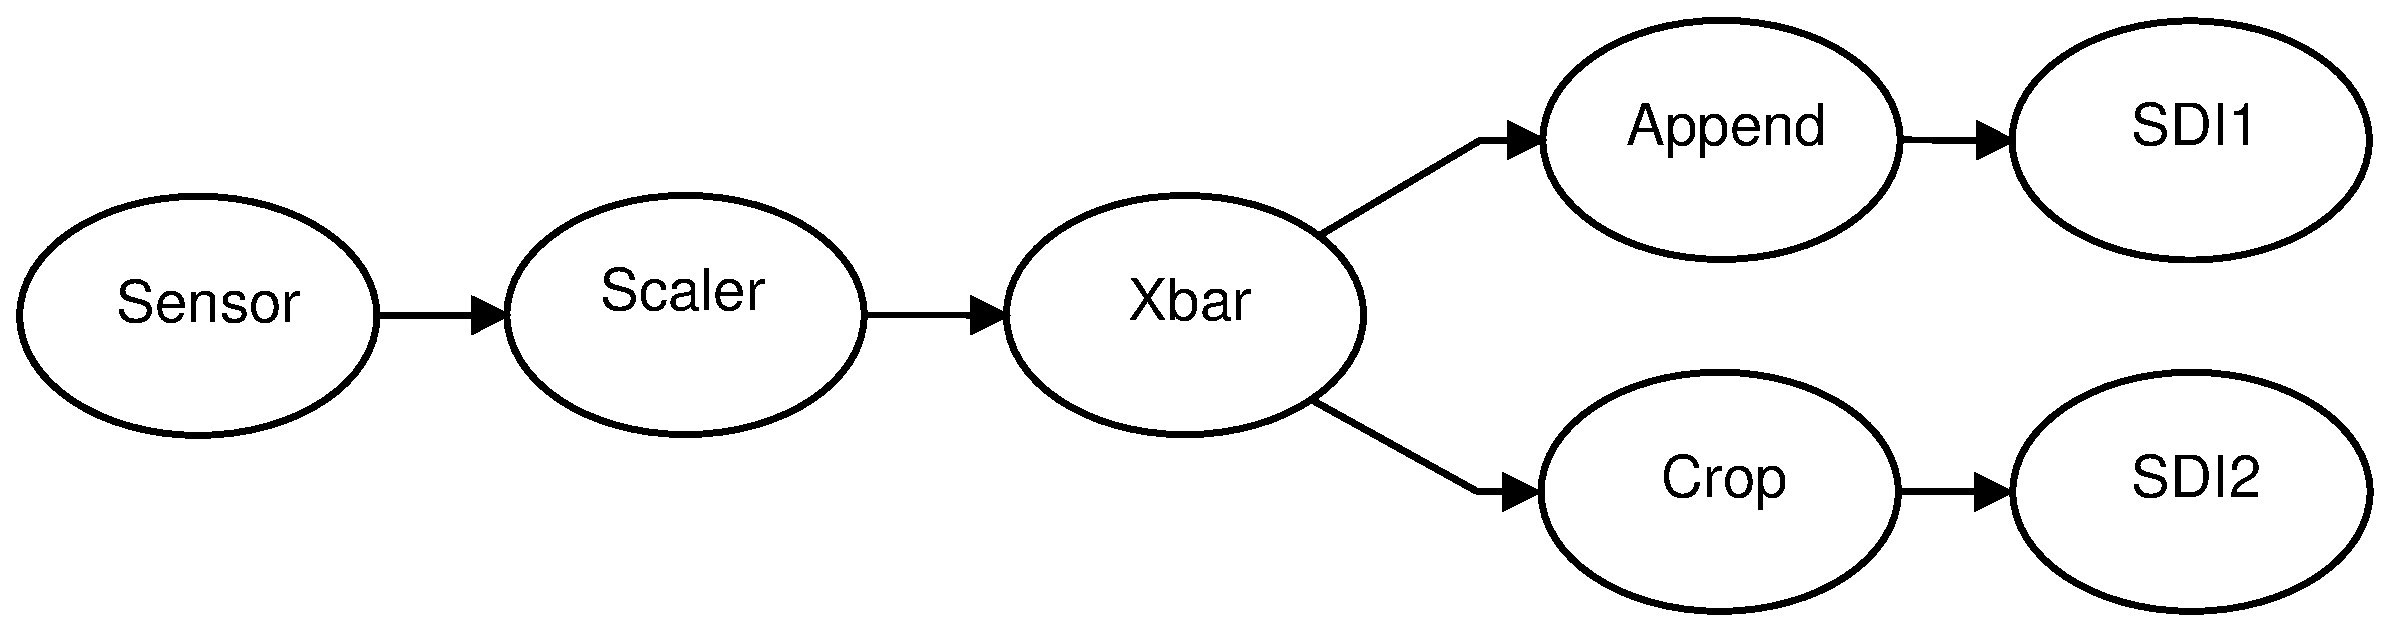
\includegraphics[width = \linewidth]{pictures/Bildkette.eps}
%	\smallskip
%	\caption{Schematische Bildkette}
%	\label{fig:bildkette}
%\end{figure} 

%In der Abbildung \ref{fig:bildkette} sieht man eine schematische Bildkette, die in diesem Bericht zur Veranschaulichung weiter detailliert wird. Das Bild an den \ac{sdi} Ausgängen wird durch verschiedene Module geleitet und angepasst. Auf die Funktionsweise der Module \ac{xbar}, Scaler, Crop sowie Append und die Implementierung wird in den nächsten Unterkapiteln eingegangen.

%\section{Funktionsweise der Module}
%Module: Scaler, Framebuffer, Append, Xbar, Crop, Resize
%Scaler: Berechnung des Bilds aufgrund des angegebenen Skalierungsverhältnis
%Xbar: Verbinden von verschiedenen Pfaden
%Append: Anpassen des Bild auf eine bestimmte Größe, dazufügen
%Crop: Anpassen des Bild auf eine bestimmte Größe, wegschneiden
%Im \ac{FPGA} sind verschiedene Module programmiert und vorkonfiguriert. Um die Kamerasoftware zu vereinfachen werden die Module auch dort angelegt.

%In diesem Abschnitt soll näher auf die Funktionsweise der einzelnen Module eingegangen werden, bevor sich der nächste Abschnitt mit der Programmierung auseinander setzt.

%Im Allgemeinen werden alle Module softwareseitig nur beschrieben, die Algorithmen der einzelnen Module sind im \ac{FPGA} verankert.

%Als erstes wird die \ac{xbar} erläutert. In diesem Modul finden keine Berechnungen statt. Durch entsprechende Konfigurationen kann die \ac{xbar} Bildpfade teilen und auch wieder zusammenfügen.

%Um das Ausgangsbild auf die richtige Größe zu skalieren wird ein Scaler eingesetzt. Hierzu wird dem Scaler ein Skalierungsverhältnis übergeben und das Modul berechnet selbstständig die richtige Ausgangsgröße.

%Die letzten beiden betrachteten Module sind von der grundsätzlichen Idee ähnlich. Durch beide Module soll das Eingangsbild auf eine bestimmte Ausgangsgröße angepasst werden. 
%Der Crop verringert die Eingangsgröße auf die Ausgangsgröße. Im Gegensatz dazu erweitert das Append die Eingangsgröße in dem ein schwarzer Rahmen um das Bild hinzugefügt wird.

%\section{Programmierung der Module}

%Für die Auswahl einer geeigneten Programmiersprache muss berücksichtigt werden, dass jedes Modul über die gleichen Eingangs- und Ausgangsgrößen verfügt. Deswegen bietet sich für \ac{geo} die objektorientierte Programmiersprache C++ an. 

%Um die spezifischen Module möglichst weit zu vereinfachen gibt es vier Grundklassen, die aufeinander aufbauen und im folgenden erklärt werden. Die Eingangsgröße soll später vom Sensor zum SDI durchgereicht werden und die Ausgangsgröße vom SDI zum Sensor. 

%\begin{figure}[!hbtp]
%	\centering
%	\includegraphics[width = \linewidth]{pictures/uml.jpg}
%	\smallskip
%	\caption{UML Übersicht der Grundklassen}
%	\label{fig:uml}
%\end{figure} 

%Die Klasse Port wird von allen anderen Klassen verwendet (siehe Abbildung \ref{fig:uml}). Hier sind alle Eingangs- und Ausgangsgröße deklariert, sowie alle Getter Funktionen für diese Größen. Im Konstruktor der Klasse muss außerdem ein Portindex mit angegeben werden, welcher auch in den Variablen der Klasse zu finden ist.

%Die beiden friend-Klassen Inport und Outport erben alle Größen und Getter der Port Klasse. Die jeweiligen Setter werden in den Klassen definiert.
%Es wird hier in Eingangs- und Ausgangsport unterschieden, damit nur die richtigen Größen gesetzt werden können. Dadurch, dass die beiden Klassen als friend class definiert sind, können sie auf die Setter der jeweils anderen zugreifen. Für die Updatefunktionen ist dies notwendig damit die Parameter durchgereicht oder berechnete Werte an die Ein- oder Ausgänge geschrieben werden können.

%Die größte Klasse im \ac{geo} ist die Klasse Module. Jedes Modul der Bildkette erbt sein Grundgerüst von dieser Elternklasse. Ein Modul kann aus mehreren Ein- oder Ausgängen bestehen, diese Anzahl wird im Konstruktor angegeben und dementsprechend werden die Ein- und Ausgänge angelegt.

%\begin{minipage}{\textwidth}
%\begin{bash}
%this->in_count = in_count;
%this->out_count = out_count;

%for (i = 0U; i < in_count; i++)
%{
%	in_ports[i] = new in_port(this->name, (geo_port_t)i);
%}

%for (i = 0U; i < out_count; i++)
%{
%	out_ports[i] = new out_port(this->name, (geo_port_t)i);
%}
%\end{bash}
%\captionof{floatcode}{Auszug aus dem Konstruktor der Klasse Module}
%\end{minipage}

%Wie in dem obigen Codeauszug zu sehen werden die privaten Variablen der Klasse auf die angegebene Anzahl von Ein- und Ausgängen gesetzt. Anschließend werden über For-Schleifen die entsprechenden Ports angelegt.

%\begin{figure}[!hbtp]
%	\centering
%	\includegraphics[width = \linewidth]{pictures/update.png}
%	\smallskip
%	\caption{Übersicht der Updatefunktion}
%	\label{fig:update}
%\end{figure} 

%Desweiteren sind in der Klasse auch Updatefunktionen (siehe Abbildung \ref{fig:update}) für jede Größe definiert. Hier werden die Größen am Eingangsport abgefragt und an den Ausgangsport übertragen beziehungsweise am Ausgangsport abgefragt und an den Eingangsport geschrieben. 

%\subsection{\acl{xbar}}
%Das Modul hat eine wichtige Aufgabe in der Kamera. Durch die \acl{xbar} können die Daten aus einem Pfad in mehr Pfade aufgeteilt werden. 

%Damit muss die Updatefunktion der Module Klasse komplett und nicht nur zu Teilen überlagert werden. Hierzu sind ein paar der Ausgangsparameter als Bitmasken angelegt. So wird garantiert, dass auch vor einer \ac{xbar} noch nachvollzogen werden kann, welche Einstellungen an dem Ausgängen vorliegen. Dies ist vor allem bei den nachfolgenden Modulen wichtig, da diese abhängig von den Einstellungen ihre Berechnungen durchführen. 

%\begin{minipage}{\textwidth}
%\begin{bash}
%void set_config(uint32_t config);
%void connect_ports(uint32_t in_port, uint32_t out_port);
%\end{bash}
%\captionof{floatcode}{Deklaration der Konfigurationsfunktionen}
%\end{minipage}

%Die Klasse \ac{xbar} hat zudem zwei Funktionen um die Konfiguration einzustellen. Bei der einen übergibt man eine Bitmaske, welche man aus vorhandenen Defines verodern kann. Die zweite Funktion besteht aus zwei Übergabeparametern, hier gibt man direkt den Eingangs- und Ausgangsport an. Auch die Abfrage der Konfiguration kann über zwei Funktionen stattfinden. Einmal kann man alle Konfigurationen abfragen und der anderen Funktion übergibt man einen Ausgangsport und bekommt den entsprechenden Eingangsport zurück.


%\subsection{Scaler}
%Der Scaler führt Berechnungen aus um das Sensorbild auf die richtige Ausgangsgröße zu skalieren. In der Kamerasoftware wird an dieser Stelle immer nur runterskaliert. 

%Die Klasse hat noch zusätzliche Variablen, diese sind jeweils doppelt vorhanden um die Vertikale und die Horizontale abzubilden. Der Divisor und der Multipikator sind die wichtigsten Parameter. In der Klasse wird die Eingangsgröße durch den Divisor geteilt und anschließend mit dem Multipikator multipliziert. Das Ergebnis wird gerundet und an den Ausgang geschrieben. Diese Berechnungen werden wieder für die Höhe und die Breite des Bildes durchgeführt. Die Variablen werden durch einen Setter gesetzt, allerdings können sie einzeln und unabhängig voneinander abgefragt werden. 

%In dieser Klasse wird nur die Updatefunktion der Elternklasse Module für die Ausgangsgrößen überschrieben. Alle anderen Parameter werden durch das Module durchgereicht und nicht verändert. 

%\subsection{Crop}
%Um den Surround View einstellen zu können wird der Crop notwendig. Wenn diese Einstellung ausgeschalten ist, soll dass Bild am Ausgang anliegen, dass vom Medium aufgezeichnet wird. Hierzu muss das Crop Modul genau den Ausschnitt aus dem Bild ausschneiden, damit liegt am Ausgang das Recordingbild an.

%Auch bei diesem Modul sind nur die Ausgangsgrößen relevant und somit wird hier nur diese Updatefunktion überlagert. Durch die Möglichkeit der Klasse verschiedene Modi einzustellen, werden dort auch entsprechende Berechnungen durchgeführt. Durch die Modi kann man am Ausgang entweder manuell eine Größe einstellen oder die Größe auf die Ausgangsgröße einstellen lassen. Zusätzlich kann man auch das Crop deaktivieren. 

%Eine Besonderheit des Moduls im \ac{FPGA} ist, dass die Ausgangsgrößen teilweise durch eine gerade Zahl teilbar sein muss. Um dies zu garantieren, gibt es in der Klasse Funktionen, die entsprechend die berechneten Größen rundet. 


%\subsection{Append}
%An den Ausgängen sollen unter anderem auch \ac{gui} eingeblendet werden. Dazu wird das Bild kleiner skaliert als der Ausgang und anschließend muss es wieder auf die Ausgangsgröße erweitert werden. Das Append Modul fügt einen schwarzen Rahmen um das Bild, über diesen Rahmen wird die \ac{gui} gelegt. 

%Bei der Klasse kann man verschiedene Modi einstellen. Über die Modi kann man das Bild auf die Ausgangsgröße erweitern, manuell eine Größe einstellen oder das Append Modul außer Betrieb setzen.

%Das Modul überschreibt von der Elternklasse nur die Ausgangsgrößen, da keine anderen neu kalkuliert werden müssen. Des weiteren kann man nicht nur den Modi setzen, sondern natürlich auch eine Ausgangsgröße einstellen. Beim manuellen Modus wird diesen dann eingestellt. 

%Ein anderer Setter ist die Möglichkeit, die Rahmenfarbe einzustellen. Im normalen Betrieb wird nur die Farbe schwarz verwendet, allerdings muss für Entwicklungszwecke die Farbe wählbar sein.

%\section{Einbindung in die Software}
%Um das \ac{geo} in die Kamera einbinden zu können, müssen zwei Aspekte betrachtet werden. Auf der einen Seite muss man die Bildkette auch in der Software abbilden können und auf der anderen Seite muss der Zugriff auf die Module stattfinden.

%\subsection{Softwareseitige Erstellung der Bildkette}
%code anschauen
%Damit die gewünschte Übersichtlichkeit in der Software erreicht wird, muss die Bildkette nicht nur im \ac{FPGA} vorhanden sein, sondern in dem Umfang auch von der Software abgebildet werden.

%Hierzu werden die vorhandenen \ac{FPGA} - Module durch die C++ Klassen abgebildet. Zuallererst werden hier die Module angelegt und im Anschluss werden Ein- und Ausgangsport hintereinander liegender Module verbunden. Damit wird sichergestellt, dass alle Größen von der Quelle bis zur Senke gelangen, bzw. andersherum.


%\subsection{Zugriff auf die Module}
%Da die Kamerasoftware in der Programmiersprache C geschrieben ist, muss eine Ebene geschaffen werden um auf die Funktionen der C++ Module im restlichen Teil der Software zuzugreifen. 

%Die Objekte werden in C++ in einer Liste verwaltet, damit braucht man für den Funktionsaufruf nur den Modulindex und die einzustellende Grüße. 

%\begin{minipage}{\textwidth}
%\begin{bash}
%void geoif_append_set_size_append(uint32_t module_idx, struct size size_append)
%{
%	append *var;
%	if (geo_system == NULL)
%	{
%		error_msg(EH_WARNING, 
%			"Geo system not initialised.");
%		return;
%	}
%	if (geo_system->get_module(module_idx) == NULL)
%	{
%		error_msg(EH_WARNING, 
%			"No module exists index \%u", module_idx);
%		return;
%	}
%	var = (append *)(geo_system->get_module(module_idx));
%	if (var == NULL)
%	{
%		error_msg(EH_WARNING, 
%			"Module at index \%u is not append.",
%			module_idx);
%		return;
%	}

%	a->set_size_append(size_append);
%}
%\end{bash}
%\captionof{floatcode}{Funktion eines Appends für C }
%\end{minipage}

%Wie man in dem obigen Codebeispiel sieht, kann die Kamerasoftware nicht direkt auf die Module zugreifen sondern geht über eine Extrafunktion. Bei dieser und allen weiteren Funktionen wird als Erstes überprüft, ob das Modul an diesem Index, dem der Funktion entspricht. Wenn dieses nicht der Fall ist, wird die Funktion verlassen. Bei einer Übereinstimmung der Module wird in der nächsten Zeile die entsprechende Größe in diesem Modul gesetzt.

%Am Ende werden die Module in der zuvor definierten Reihenfolge geupdatet und damit sind in jedem Modul die richtigen Größen und Werte.

%\subsection{Übertragen der Größen in den \ac{FPGA}}
%Am Ende müssen die in dem \ac{geo} eingestellten Größen in die Module des \ac{FPGA}s übertragen werden. Hierzu werden die richtigen Module auf Software- und Hardwareseite zusammen aufgerufen. Die Größen des Moduls werden aus dem \ac{geo} entnommen und über entsprechende Hardwarefunktionen in die Register des \ac{FPGA}s geschrieben. An diesem Punkt findet allerdings keine Überprüfung auf die Richtigkeit des Moduls statt, sondern lediglich die Kontrolle, ob dieses im \ac{geo} und im \ac{FPGA} existiert.




\chapter{Software-Tests und Debugging} \label{sec:test}
% testbackend muss noch geschrieben werden
% überlegungen zum testen aufschreiben 

\section{Einführung}
Zum Testen der Funktionalität der Software haben sich über die Zeit Grundsätze gebildet, welche als generelle Leitlinien beim Testen gesehen werden. \citep[S. 53]{spillner2005basiswissen}
Einige Grundsätze sollen im Folgenden näher betrachet werden, dass sie für die Frameworktest essentiell sind. 

Der erste Grundsatz besagt, dass ausreichendes Testen die Wahrscheinlichkeit von Fehlerfällen im laufenden Betrieb verringert. Beim Ausbleiben von Fehlern beim Testen ist dies kein Indikator für die Fehlerfreiheit des Codes.
Im zweiten Grundsatz wird erläutert, dass vollständiges Testen nicht möglich ist. Eine Ausnahme sind die Tests bei sehr trivialen Testobjekten. 
Für die frühzeitige Erkennung der Fehler besagt der dritte Grundsatz, dass frühzeitig mit dem Testen begonnen werden soll. \citep[S. 53]{spillner2005basiswissen}


Aufgrund des zweiten Grundsatz ist es nicht möglich, dass komplette \gls{framework} zusammen zu testen. Um einfache Testobjekte zu erhalten, werden die einzelnen Module über die \ac{fra} Bibliothek getestet. Durch die Unittest der Module wird zudem die Wahrscheinlichkeit von Fehlern in diesem Bereich verringert. Außerdem sollen die Tests entsprechend mit neuen Funktionen in der Bibliothek erweitert werden, sodass die Funktionen direkt getestet werden.



Durch die \gls{unittest} können nicht alle potenziellen Fehlerfälle abgedeckt werden. Durch die Abhängigkeit der korrekten Funktionsweise der Kamera von allen Prozessen, ist einfaches Debugging mit einem entsprechenden Programm nicht möglich. In der vorhandenen Implementierung wird die Fehlersuche bereits über die Protokollierung von Meldungen in einer Datei gehandelt. Um eine schnelle und einfache Möglichkeit zu geben, die Zugriffe im \ac{fra} zu protokollieren und eventuell neue Geräte anzulegen, wird die Funktionalität in kleine Programme eingebettet. Diese sollen im laufenden Betrieb ausgeführt werden können. 



\section{Plattformunabhängige Tests}
%Hierzu sollen die modulspezifischen Funktionen mit definierten Parametern aufgerufen werden und anschließend kontrolliert werden, ob die Funktionen die richtigen Parameter weitergibt.
Zunächst soll auf die Tests eingegangen werden, die unabhängig von der Entwicklungsumgebung durchgeführt werden können. 
Dafür werden \gls{unittest} für jedes  Modul angelegt. Dadurch kann die Funktionalität der einzelnen Module überprüft und im Fehlerfall direkt gehandelt werden. Vor allem bei Änderungen an der \ac{fra} \gls{middleware} und Bibliothek können so vor der Inbetriebnahme auf der Kamera Fehler gefunden und ausgebessert werden.


Im \gls{unittest} wird die virtuelle Hardware angelegt und geöffnet, anschließend werden modulspezifische Funktionen aufgerufen und direkt danach der Check durchgeführt. Der Ablauf eines \gls{unittest} ist in Abbildung~\ref{fig:testbackend} dagestellt und wird im folgenden näher erläutert.


\begin{figure}[!hbtp]
	\centering
	\includegraphics[width = \linewidth]{pictures/2019-11-28-testbackend.png}
	\smallskip
	\caption{Beispielhaftes Sequenzdiagramm zum \gls{unittest}}
	\label{fig:testbackend}
\end{figure} 


\begin{lstfloat}
\begin{lstlisting}
struct fra_test_mod
{
	char type[FRA_MAX_NAME];
	char name[FRA_MAX_NAME];
	uint32_t size;
	uint32_t *reg;
};
\end{lstlisting}
\captionof{code}{\label{code:fra_test_mod} Struktur zum Abbilden der virtuellen Hardware}
\end{lstfloat}

Durch das Anlegen eines Geräts im Kernelbackend können alle benötigten Informationen und Register über dieses Gerät abgefragt und gesetzt werden. Da das Testbackend unabhängig funktionieren soll, ist das Anlegen von Geräten so nicht möglich. Um eine ähnliche Funktionalität wie im Kernel zu haben, wird das Modul über die \textit{fra\_mod\_test} Struktur abgebildet. Hier werden alle notwendigen Informationen angelegt und auch entsprechende Register abgebildet, damit man diese beschreiben und auch auslesen kann.
Die \textit{fra\_mod\_test} Struktur wird als statisches Array im Testbackend angelegt und bildet so die virtuelle Hardware für das Testprogramm. Dadurch ist das Überprüfen der Register später möglich und auch eine maximale Anzahl der Module ist vorgegeben. 


Damit die virtuelle Hardware richtig initialisiert wird, muss für die Register entsprechender Speicherplatz allokiert, aber auch die restlichen Parameter gesetzt werden. Analog dazu muss der Speicherbereich der Register beim Beenden des Programms wieder freigegeben werden. Dafür gibt es im Testbackend zusätzliche Funktionen, die sich um das initialisieren (\textit{fra\_test\_init}) und deinitialisieren(\textit{fra\_test\_deinit}) kümmern.\\

 
Beim Starten des Test werden der \textit{fra\_test\_init} Funktion drei Parameter übergeben. Zum Einen wird der Name sowie der Typ des Moduls und zum Anderen wird die Größe des Registers in die Funktion gereicht. Ist die maximale Anzahl der Module noch nicht überschritten, wird mithilfe der Größe ein Registerblock allokiert. Anschließend wird die \textit{fra\_mod\_test} Struktur mit allen vier Parametern gefüllt und eine statische Variable \textit{mod\_count} erhöht.

Wenn der Test am Ende angelangt ist, werden in der \textit{fra\_test\_deinit} Funktion mithilfe der Variablen \textit{mod\_count} alle allokierten virtuellen Geräte wieder freigegeben.\\


Zum Öffnen eines Moduls im Testbackend wird analog zum Kernelbackend die Funktion \textit{fra\_init} aufgerufen. Hier wird allerdings ein anderer Backendtyp übergeben und somit in den Wrapperfunktionen entsprechend ins Testbackend weitergeleitet. 
Die Funktionalität der einzelnen Backendfunktionen ist, im Vergleich zum Kernelbackend, vereinfacht worden und die Funktionen kommen entsprechend ohne \ac{ioctl}s aus. Das Setzen und Lesen der Register erfolgt nun über die \textit{fra\_mod\_test} Struktur im \gls{handle}. Diese wird bei der \textit{fra\_test\_open} Funktion als Zeiger auf die entsprechende Stelle im statischen \textit{fra\_mod\_test} Array beschrieben. Die richtige Stelle wird über einen Vergleich mit dem Modulname gefunden.\\



Damit überprüft werden kann, ob die Register richtig beschrieben bzw. ausgelesen worden sind, gibt es zwei Funktionen. Diese sind, wie die \textit{fra\_test\_init} und \textit{fra\_test\_deinit} Funktion, im Testbackend, aber werden ohne Wrapperfunktion aufgerufen, da sie spezifisch sind und lediglich beim Testen benötigt werden.
Der \textit{fra\_test\_check} Funktion werden neben dem \gls{handle} noch die Registernummer und der Sollwert des Registers übergeben. Über den Namen wird die Zuordnung des \glspl{handle} zu der virtuellen Hardware gemacht und anschließend der Registerwert mit dem Sollwert verglichen. Bei einem fehlerhaften Wert wird eine Fehlermeldung ausgegeben und der Rückgabewert ist 1.
Durch eine weitere Funktion (\textit{fra\_test\_check\_all}) kann das gesamte Registerset überprüft werden. Allerdings muss hier neben dem \gls{handle} noch ein Array der Registergröße übergeben werden. In diesem Array müssen die Sollwerte in richtiger Reihenfolge gespeichert sein. Anschließend wird für jede einzelne Registerstelle die \textit{fra\_test\_check} Funktion aufgerufen. Am Ende wird die Gesamtanzahl der Fehler zurückgegeben, welche im Test ausgewertet wird.\\




\section{Tools für die Zielplattform}
Unabhängig von den Funktionstests des vorherigen Kapitels sollten dem Entwickler kleine Programme zur Verfügung gestellt werden, mit denen man für Testprogramme oder zur Fehlersuche im laufenden Betrieb ein Gerät anlegen oder das Logging aktivieren kann. \\


Besonders für die Kalibrierung der Kamera ist es notwendig ein Gerät über die Kommandozeile anzulegen, da es hier keinen Codeteil gibt, in welchem das Anlegen integriert werden könnte. Dadurch, dass die benötigten Geräte vor dem Starten der Kalibiersoftware angelegt werden, können in der Software über die Funktionen der \ac{fra} \gls{middleware} und Bibliothek die Geräte geöffnet und auf diese zugegriffen werden.


Beim Ausführen des Programms \textit{fra\_create\_device} werden in der Kommandozeile über Optionen die benötigten Parameter übergeben. Hier gibt es, neben dem Namen, dem Typ, der Adresse und der Größe auch die Möglichkeit eine Hilfe auszugeben, in welcher genauer erläutert wird, wie das Programm zu nutzen ist. 
Nach dem Ausführen des Programms werden die programminternen Parameter mithilfe der Optionen gefüllt und nach der Überprüfung auf Dateninkonsistenz wird das entsprechende Gerät angelegt. 
Danach ist dieses Gerät in Linux unter \textit{dev/fra/} zu finden und weitere Programme oder Testtools können darauf zugreifen.\\

Ein weiteres nützliches Tool für die Entwicklungsarbeit ist das \textit{fra\_set\_logging}. Da das Logging standardmäßig deaktiviert ist, muss dieses bei Bedarf aktiviert werden. Damit der Entwickler nicht im entsprechenden Code die Aktivierung vornehmen und zeitaufwendig neu kompilieren muss, wird durch das Testtool ein entsprechendes Werkzeug bereitgestellt. Durch das Programm kann im laufenden Betrieb der Kamera die Protokollierung eines Geräts aktiviert oder deaktiviert werden.


Hier werden beim Starten des Programms auf der Kommandozeile entsprechend den Optionen der Name des Geräts und ein Setparameter übergeben. 
Über den Setparameter wird entschieden, ob das Logging aktiviert (\textit{set=1}) oder deaktiviert (\textit{set=0}) werden soll. Anschließend wird das Gerät über den Namen geöffnet und über das entsprechende \ac{ioctl} wird das Logging gesetzt. Nach dem Schließen des Geräts wird das Programm beendet. \\


Beide Tools sind für den Einsatz auf der Zielplattform gedacht und sollen Entwicklern und Testern vor allem die Fehlersuche auf der Kamera erleichtern. Bei Bedarf können die Programme einfach erweitert werden oder weitere Tools in Anlehnung an die Codestruktur geschrieben werden. 
\chapter{Fazit und Ausblick}
% Transaktionsids
% Bild Anton
%Die Abhängigkeit von einem händisch eingetragenen Offset ist so immer noch vorhanden!!!
% weitere vorgehensweise, weitere module, speicherbereiche, arbeitsaufwand: ca halbes jahr

In diesem Kapitel soll ein Fazit über das in der Arbeit behandelte \ac{fra} gezogen werden und zusätzlich ein Ausblick auf die weitere Vorgehensweise zur Einbindung in die Software und notwendige Erweiterungen gegeben werden.


\section{Zusammenfassung der Ergebnisse}
%letzes framework zum umstrukturieren der software, 
% abstraktion zur hardware, kein direkter zugriff mehr
% testen möglich
% über verschiedene ebenen

Ein wichtiger Punkt für das \ac{fra} war die Abstraktion der Hardware. Durch die direkten Zugriffe von der Kamerasoftware auf den \ac{fpga} ist die Fehlersuche recht zeitaufwendig gewesen. Durch das neue Framework wird nicht mehr über direkte Adressen auf die Hardware zugegriffen. Dadurch ist es einfacher nachzuvollziehen, aus welchem Prozess die Funktionsaufrufe kommen und kann so im Fehlerfall auch einfach protokolliert werden.


Des weiteren wird durch die Einteilung in drei verschiedene Ebenen im Userspace eine einfache Möglichkeit gegeben um Tests zu implementieren. Durch das Testbackend und die \ac{fra} Middleware können die modulspezifischen Funktionen identisch wie in der Kamerasoftware aufgerufen werden und somit überprüft werden, ob die \ac{fra} Bibliothek richtig funktioniert. So können durch die Unittests bei jeder Neuerung und Änderung in der Bibliothek oder Middleware frühzeitig Fehler gefunden und behoben werden.


Durch das \ac{fra} ist der letzte Schritt in einer Umstrukturierung der Software gemacht worden. Die letzten Jahre wurde die Software bereits funktional durch die Implementierung des \ac{geo} abstrahiert. Durch das Zusammenspiel der beiden Abstraktionsebenen ist es nun möglich ohne tiefere Kenntnisse von \ac{fpga} und Bildkette die Kamerasoftware durch unterschiedliche Entwickler zu Pflegen und zu Erweitern.


\section{Ausblick}
%weitere vorgehenesweise: restliche module umziehen, speicherbereiche im fpga von modulen umziehen: ca halbes jahr
%tests weiter ausbauen

%abhängigkeit von händischen offset noch vorhanden, muss noch raus
% transids mit funktionalität belegen

Damit des \ac{fra} vollständig in der Software eingebunden ist, müssen noch weitere Schritte gemacht werden. Zum Einen müssen die restlichen Module der Bildkette samt ihrer spezifischen Funktionen in die \ac{fra} Bibliothek umgezogen werden und zum Anderen haben ein paar Module in \ac{fpga} Speicherbereiche um die Bilder zwischen zu speichern, auch diese müssen für die komplette Umstellung im \ac{fra} abgebildet werden. Der Arbeitsaufwand für den kompletten Umzug der Software auf das Framework wird auf ungefähr ein halbes Jahr geschätzt.

Auch die Abhängigkeit von händisch eingetragenen Adressen ist noch immer vorhanden (siehe Kapitel~\ref{sec:konzept}). Diese soll in Zukunft durch ein generisches Modell ersetzt werden und somit eine komplette Unabhängigkeit von den \ac{fpga} Adressen in der Software schaffen. Dies ist vor allem in Anbetracht der Wartbarkeit der Software ein wichtiges Thema.

Wie in Kapitel~\ref{sec:middleware} erwähnt, wird in der aktuellen Implementierung des \ac{fra} die Transaktionsidentifikation durch alle Funktionsaufrufe durchgereicht. Bei bestimmten Teilen der Bildkette hängen die Einstellungen der Module stark voneinander ab, aus diesem Grund ist es sinnvoll die Zugriffe auf die Module zu gruppieren. Dadurch können die \ac{fpga} Zugriffe direkt hintereinander aufgerufen werden und so Bildfehler vermieden werden.


















%In diesem Abschnitt soll auf die weitere Verwendung des \ac{geo} eingegangen werden und ein Ausblick auf die Zukunft gegeben werden.

%\section{Zum \ac{geo}}
%Zu Beginn von Kapitel \ref{sec:haupt} wurde schon erwähnt, dass es mehr Module als die vier in der Arbeit betrachteten Module gibt. Aktuell gibt es um die zehn verschiedenen Module, allerdings werden, außer zu Entwicklungszwecken, keine neuen Module dazukommen. 
%In der Kamerasoftware existieren noch viele Stellen an der die betrachtete Abstraktionsebene gar nicht oder nicht vollständig zum Einsatz kommt. Natürlich soll das \ac{geo} an allen möglichen Stellen verwendet werden. Aus diesem Grund müssen die unterschiedlichen Module entweder einzeln oder übergreifend um neue Parameter erweitert werden. Auch die modulspezifischen Abhängigkeiten müssen weiter angepasst und gepflegt werden. 

%Insbesondere müssen hardwareseitige Änderungen berücksichtigt werden und entsprechend softwareseitig die Module nachgezogen werden.
%\section{Über die betrachtete Abstraktionsebene hinaus}
%Zur weiteren Verbesserung der Software soll es in Zukunft noch eine weitere Abstraktionsebene geben. Diese sogenannte \ac{fra} soll dann allerdings nicht wie das \ac{geo} die Bildkette abbilden, sondern die Hardwarefunktionen aus der Hauptcode elimentieren und damit für noch mehr Wartbarkeit sorgen. 

%Durch das Zusammenspiel der beiden Abstraktionsebenen soll ohne tiefere Kenntnisse von \ac{FPGA} und Bildkette das Pflegen und Erweitern der Kamerasoftware durch unterschiedliche Entwicklern ermöglicht werden.

\printbibliography[title=Literaturverzeichnis]

%% Beim Anhang gibt es eine Musterdatei, die 
%% erg�nzt werden kann
\appendix
\chapter*{Anhang\markboth{Anhang}{Anhang}}
\setcounter{chapter}{1}
\addcontentsline{toc}{chapter}{Anhang}

\printindex
\printbibliography[title=Literaturverzeichnis, sorting=nyt, heading=subbibnumbered]
%Abbildungsverzeichnis
\listoffigures
%Tabellenverzeichnis
\listoftables


%% Stichwortverzeichnis ausgeben.
%% falls nicht notwendig, die folgende Zeile loeschen
\printindex

\end{document}
